\subsection{Systemarchitektur}\label{subsec:systemarchitektur}
\subsubsection*{Abgrenzung}

Dieses Kapitel gibt einen Übersicht über die Systemarchitektur als ganzes. Die Architektur beschränkt sich dabei auf die
Anforderungen die innerhalb des Projektrahmens umgesetzt wurden. Komponenten für Teile die Out Of Scope gefallen sind,
werden hier nicht behandelt.

\subsubsection*{Übersicht}

Das cloudbasierte Praxisrufsystem wird in vier Komponenten unterteilt.
Im Zentrum steht eine cloudbasierte Applikation (Cloud Service) welche es ermöglicht Konfigurationen persistent zu verwalten und das Versenden von Benachrichtigungen anhand dieser Konfigurationen koordiniert.
Der Cloud Service benutzt einen externen Messaging Service zum Versenden von Benachrichtigungen. Dabei ist der Messaging Service lediglich für die Zustellung von Benachrichtigungen verantwortlich.
Zur Verwaltung der Konfigurationen wird ein Web Frontend (Admin UI) erstellt. Dieses bietet einem Administrator die Möglichkeit Konfigurationen aus dem Cloud Service zu lesen, erstellen, bearbeiten und löschen.
Die Konfigurationen die über Admin UI und Cloud Service erstellt wurden, werden schliesslich von einem Mobile Client. Mit dem Mobile Client kann der Benutzer Benachrichtigungen an andere Mobile Clients senden.
Welche Benachrichtigungen ein Mobile Client senden kann und an wen diese Benachrichtungen zugstellt werden, wird anhand der Konfiguration aus dem Cloud Service bestimmt.

\begin{figure}[h]
    \centering
    \begin{minipage}[b]{1.0\textwidth}
        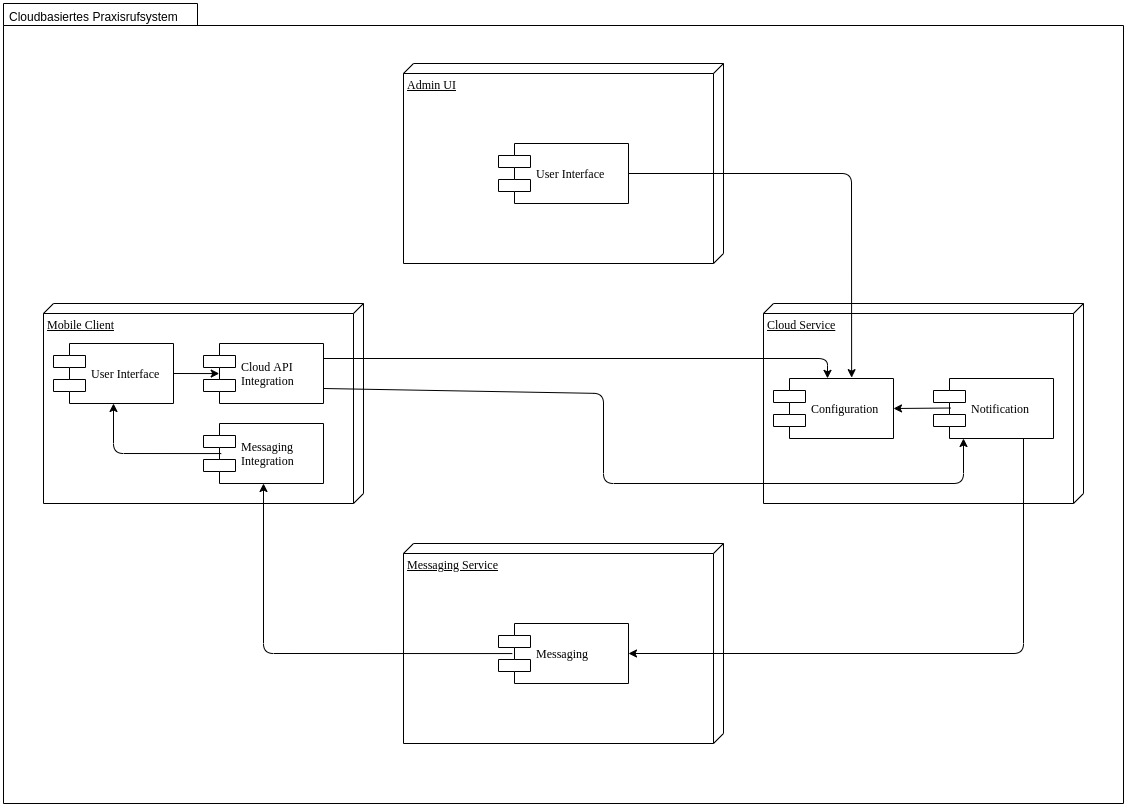
\includegraphics[width=\textwidth]{graphics/Component_System}
        \caption{System}
    \end{minipage}
\end{figure}

\clearpage

\subsubsection*{Mobile Client}

Damit der Praxismitarbeiter wie in den Anforderungen U01 und U02 beschrieben Benachrichtigungen versenden und empfangen kann,
benötigt das System einen Client, welcher dem Praxismitarbeiter diese Oprationen ermöglicht. Die technischen Anforderungen
T01, T02 und T03 setzen voraus, dass dieser Client über die Mobil Geräte (IPads und Android Tablets) bedient werden kann.

\begin{itemize}
    \item T01
    \item T02
    \item T03
    \item U01
    \item U02
    \item U03
    \item U04
    \item U05
    \item U06
    \item U07
\end{itemize}

\subsubsection*{Cloud Service}

Der Cloud Service ermöglicht Konfigurationen persistent zu verwalten und das Versenden von Benachrichtigungen anhand dieser Konfigurationen koordiniert.
Der Cloud Service benutzt einen externen Messaging Service zum Versenden von Benachrichtigungen.

\begin{itemize}
    \item U01
    \item U02
    \item U03
    \item U06
    \item U07
\end{itemize}


\subsubsection*{Messaging Service}

Der Messaging Service ist für die Zustellung von Benachrichtigungen verantwortlich.

\begin{itemize}
    \item U01
    \item U02
    \item U03
    \item U04
    \item U06
\end{itemize}

\subsubsection*{Admin UI}

Damit der Praxisverantwortliche die Konfiguration des Praxisrufsystems verwalten kann ist es notwendig, dass alle
Lese und Schreib Zugriffe auf die Konfiguration über eine Zentrale Stelle gehen, auf die der Praxisverantwortliche Zugriff hat.

\begin{itemize}
    \item U12
    \item U13
    \item U14
    \item T04
\end{itemize}

\clearpage
